\section{Computer Images}

\begin{frame}[fragile]
  \frametitle{What is an image?}
  An image is made up of pixels. Each pixel is a number. Computers
  store images as matrix of numbers.\\
  \vspace{3mm}
  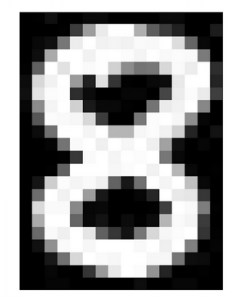
\includegraphics[scale=0.4]{img/img_1}
  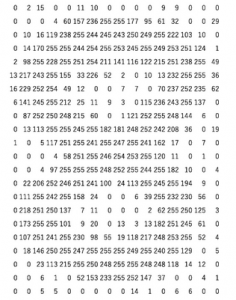
\includegraphics[scale=0.4]{img/img_2}\\
  \vspace{3mm}
  The dimension of an image is n x m. This is the number of pixels
  in the image (height x width).\\
  Each number could represent a color or intensity/brightness (black and white).
\end{frame}

\begin{frame}[fragile]
  \frametitle{Colored image}
  A colored image has 3 matrices, red, green and blue. Each matrix has
  values between 0 and 255, representing the intensity of the color in that
  pixel.\\
  \vspace{3mm}
  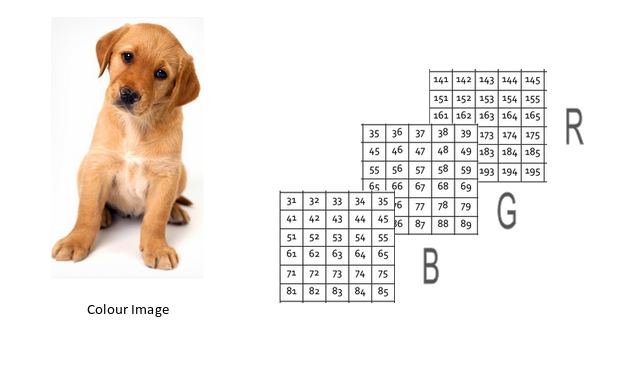
\includegraphics[scale=0.4]{img/img_3}
\end{frame}

\begin{frame}[fragile]
  \frametitle{Thin Blood Smear Image}
  \verb|https://lhncbc.nlm.nih.gov/publication/pub9932|\\
  \vspace{3mm}
  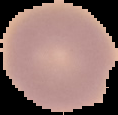
\includegraphics[scale=1]{img/img_4}\\
  \vspace{3mm}
  Dimension: 115 x 115 x 3
\end{frame}

\begin{frame}[fragile]
  \frametitle{Feature Extraction}
  Extract useful information of the image content.
\end{frame}
